\documentclass[12pt]{exam}
\usepackage[top=2cm, bottom=3cm, left=2cm, right=2cm]{geometry}
\usepackage{graphicx}
\usepackage{amsmath,amsfonts,amssymb,amsthm}
\usepackage{yhmath} % \wideparen
\usepackage[colorlinks=true, linkcolor=brown, urlcolor=brown]{hyperref}
\usepackage{xeCJK}
\usepackage{xcolor}
\usepackage{float}
\usepackage{enumitem}
\usepackage{tikz}
\usetikzlibrary{calc}
\usepackage{mathtools}
\usepackage{lipsum}
\usepackage{pgfornament}
\usepackage{multicol}
\usepackage{worldflags}
\usepackage{pifont}
\usepackage{ifthen}
\usepackage{booktabs}
\usepackage{tabularx}
\usetikzlibrary{shapes.geometric, positioning}
\setCJKmainfont{KaiTi}

%\includeonly{微积分}
%\includeonly{离散数学}
%\includeonly{几何}
%\includeonly{代数}
\includeonly{统计学}
%\includeonly{证明手册}
%\setCJKmainfont[BoldFont=Noto Sans CJK SC Bold]{AR PL KaitiM GB} 

%\begin{solution}
    %\textcolor{red}{(待验证)}
%\end{solution}

%ifprintanswers
%\begin{figure}[H]
    %\centering        
    %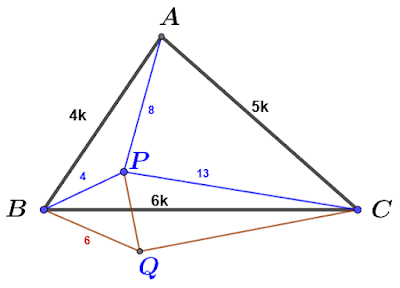
\includegraphics[width=0.5\textwidth]{images/image25.png}
%\end{figure}[]
%\fi

%output copyable code snippet: 简体字版本latex code的copyable code snippet,注意一定要简体字,以\question开始然后才\begin{solution},请完全按照原文,有小题的话用\question \begin{parts}然后一小题\part accompanied by 一个\begin{solution},dx之前要用\,,用\[...\]或\begin{align*}或$...$但不要用$$...$$,\[...\]里不能放\begin{align*},\[然后下一行content然后下一行\],用\frac{}{}不要a/b,中文字不可以在\[...\]里面,不要用\text{中文字},不要用\textbf{},\boxed及\ans,不要用\overline{},句号。不要在\[...\]里面,如果有\frac{}{}在brackets里要\left(...\right)
%有小题的话用\question \begin{parts}然后一小题\part accompanied by 一个\begin{solution},dx之前要用\,,把这些⑦变为(7)
%when i give ss, only provide the code for the new ss, do not output for all the previous one
%give copyable latex code for every screenshot i provide
%give copyable latex code in a chunk&
%write into single line of \[...\] with ,\quad in between
%put into single \[...\] with \Rightarrow in between
%write into begin align*

%unexplored/to expand later areas: 
%统计学-H2 maths p2 - prob distribution & hypo testing
%vietnam exam
%korea exam
%singapore exam
%hongkong exam
%上海师范大学-数理逻辑
%madas maths advanced topics - diff under the integral sign,diagonalization_of_conics_and_quadrics, intrinsic_coordinates
%不等式-放缩法、数形结合、赫尔德不等式、琴生不等式
%解三角形-已知五心/两条垂线/两条中线及两点/两线求第三点/线、对称点公式、塞瓦定理
%圆-两圆正交,两圆公切线
%矩阵-adjadj, detadjadj
%平面向量-vector证明whatsapp 29 Jan,u\cdot v^hat=u^hat\cdot v,projection matrices are idempotent and symmetric
%linear algebra线代启示录
%华罗庚-初中几何题
%MOS Vol 8 - Appendix Proof
%AMC 10-包括数论
%指考,APMO,SEAMO,CTMC,CSMC,台湾,中国
%integral marathon, integration bee
%https://www.youtube.com/@johnlu9432/playlists

%大排版/clean up issues:
%关键词
%跟着solution排版
%由易至难/跟着课文走?跟着课文走+综合题/挑战题
%难度:眼光、麻烦、雾里看花、课外太空
%函数的递推题丢去数列
%三角不等式放哪?
%数列里有用到复数?
%圆锥曲线
%三角恒等式?
%参数化积分放哪？
%边长去掉|...|for |AB|,保留for|\vec{AB}|
%不等式要等号成立条件
%极限、微分move to 积分
%向量、空间几何
%不定积分要加C
%积分太乱了
%离散数学-数理逻辑、计数原理、排列与组合

%统计学-
%概率
%随机变量(discrete: binomial,poisson,geometric, hypergeometric, continuous random variables, probability density function, cumulative distribution function, expectation and variance of uniform, normal, N(0,1),exponential, gamma,联合分布(joint distribution)
%期望值(covariance,correlation、moment generating functions)
%假设检验

%fixed issues:
%余弦定理求边时打横写
%\mathbb{R}显示不正常,但如果comment out \usepackage{amsmath, amssymb, amsfonts} 就不能放\square,
%\mathbb{R}显示不正常,\setmathfont{TeX Gyre Termes Math} for \unicodemath,but not compatible with xelatex? - \usepackage{yhmath} for \wideparen
%inverse trig,differential equations
%微分方程步骤中间用小写c, 最后答案用大C - C_1,C_2,...
%若指数为一积分,用exp()
%裂项求和-> 累加法/累乘法
%limit的泰勒展开

\newcommand{\ans}[1]{{\color{blue}#1}}
\newcommand*{\perm}[2]{{}^{#1}\!P_{#2}}
\newcommand*{\comb}[2]{{}^{#1}C_{#2}}
\newcommand{\parallels}{\mathbin{\!/\mkern-5mu/\!}}
\newcommand{\congr}{\ \reflectbox{$\cong$} \ }
\renewcommand{\ge}{\geqslant}
\renewcommand{\geq}{\geqslant}
\renewcommand{\le}{\leqslant}
\renewcommand{\leq}{\leqslant}
\DeclarePairedDelimiter\ceil{\lceil}{\rceil}
\DeclarePairedDelimiter\floor{\lfloor}{\rfloor}
\newcommand{\separator}{% 
  {\par\noindent
  
\begin{tikzpicture}
    \coordinate (C) at (0,0);
    \coordinate (D) at (\textwidth,0);
    \path (C) to[ornament=88,options/.append style={yshift=.52pt,scale=0.8}] (D);
  \end{tikzpicture}}
}
\newcommand{\rating}[1]{%
    \text{\ding{72}}%
    \ifthenelse{#1 > 1}{\text{\ding{72}}}{\text{\ding{73}}}%
    \ifthenelse{#1 > 2}{\text{\ding{72}}}{\text{\ding{73}}}%
    \ifthenelse{#1 > 3}{\text{\ding{72}}}{\text{\ding{73}}}%
    \ifthenelse{#1 > 4}{\text{\ding{72}}}{\text{\ding{73}}}%
}
\printanswers
\shadedsolutions
\definecolor{SolutionColor}{rgb}{1.0,0.98,0.8} %https://latexcolor.com/
\definecolor{PageColor}{rgb}{1.0,0.98,0.8}
\renewcommand{\solutiontitle}{\noindent}
\solutionsreseteqcounter
%\SolutionEmphasis{\color{red}}
\linespread{1.3}
\flagsdefault[width=0.5cm]
\setlength{\footskip}{0.5cm} 
\setlength{\columnsep}{1cm}
\newcommand{\figureornament}[2][1]{\raisebox{.5\fontcharht\font`0}{\pgfornament[scale=#1,color=brown]{#2}}}
\footer{}{- \;\thepage \; -}{} 
%\runningfooter{}{\figureornament[0.2]{11}\;\; \thepage \;\; \figureornament[0.2]{14}}{}

\begin{document}
\input{titlepage}
\thispagestyle{empty} %clear away page 1
\begin{center}
  {\fontsize{30pt}{26pt}\selectfont 前言
  }
\end{center}
\vspace{1cm}

\begin{tikzpicture}[every node/.style={inner sep=0pt}]
\node[text width=11.5cm](Text){%
\qquad 追溯到 2019 年,为了当年的备赛,我疯狂爬取 AMC 历届考题,整出了《AMC 10 精选》和一份“统考超纲难题集”。直到2025 年5月,我看着当年的内容不禁感叹:读了数学系之后,总觉得这里的发展空间实属不少。这些日子,我开启了采集模式,在网上搜刮各种有趣（恶心）、深奥（烧脑）的题目。\\[10pt]

\qquad 本来没打算写解析,但发现很多老题只有答案。我的大脑停工了一年,有些题连现在的我读起来都觉得难以下咽,是不是百尺竿头,更蠢一步。为了不让未来的自己看到题目时再次怀疑人生,我决定用 \LaTeX{} 重新排版,并含泪补全了解法,最终整出了这份——《高级数学 (III) 训练集》。\\[10pt]

\qquad 为此,我广泛参考了美、加的数学竞赛,日、印的大学入学考,以及台湾的教师甄选题,等等。尽管整理过程艰辛,但也领略了全球不同地区的数学教纲,宛如经历了一场“数学环游世界”。\\[10pt]

\qquad 建议想自己动手的朋友,可在 \texttt{preamble} 中注释掉 \verb|\printanswers|。解析皆来自官方或亲笔,但绝大部分也经 \texttt{ChatGPT,Gemini}修改,若有纰漏欢迎指正。祝大家阅读愉快！\\[10pt]
\hfill —— 冬恒} ;
\color{brown}
\node[shift={(-1.5cm,1.5cm)},anchor=north west](CNW)
at (Text.north west) {\pgfornament[width=1.75cm]{61}};
\node[shift={(1.5cm,1.5cm)},anchor=north east](CNE)
at (Text.north east) {\pgfornament[width=1.75cm,symmetry=v]{61}};
\node[shift={(-1.5cm,-1.5cm)},anchor=south west](CSW)
at (Text.south west) {\pgfornament[width=1.75cm,symmetry=h]{61}};
\node[shift={(1.5cm,-1.5cm)},anchor=south east](CSE)
at (Text.south east) {\pgfornament[width=1.75cm,symmetry=c]{61}};
\pgfornamenthline{CNW}{CNE}{north}{87}
\pgfornamenthline{CSW}{CSE}{south}{87}
\pgfornamentvline{CNW}{CSW}{west}{87}
\pgfornamentvline{CNE}{CSE}{east}{87}
\end{tikzpicture}

\pagebreak
\begin{center}
  {\fontsize{30pt}{26pt}\selectfont 目录
  }
\end{center}
\separator

\begin{multicols}{2}
\begin{center}
    {\Large 代数}
\end{center}
\hyperlink{一元二次方程、多项式}{一元二次方程、多项式} \dotfill \pageref{一元二次方程、多项式} \\
\hyperlink{因式定理、余式定理}{因式定理、余式定理} \dotfill \pageref{因式定理、余式定理} \\
\hyperlink{无理式、绝对值}{无理式、绝对值} \dotfill \pageref{无理式、绝对值} \\
\hyperlink{指数与对数}{指数与对数} \dotfill \pageref{指数与对数} \\
\hyperlink{方程组}{方程组} \dotfill \pageref{方程组} \\
\hyperlink{函数}{函数} \dotfill \pageref{函数} \\
\hyperlink{不等式、最值问题}{不等式、最值问题} \dotfill \pageref{不等式、最值问题} \\
\hyperlink{数列、级数}{数列、级数} \dotfill \pageref{数列、级数} \\
\hyperlink{二项展开式}{二项展开式} \dotfill \pageref{二项展开式} \\
\hyperlink{泰勒展开式}{泰勒展开式} \dotfill \pageref{泰勒展开式} \\
\hyperlink{矩阵}{矩阵} \dotfill \pageref{矩阵} \\
\hyperlink{行列式}{行列式} \dotfill \pageref{行列式} \\
\hyperlink{复数}{复数} \dotfill \pageref{复数}
\begin{center}
    {\Large 几何}
\end{center}
\hyperlink{三角形}{三角形} \dotfill \pageref{三角形} \\
\hyperlink{三角函数}{三角函数} \dotfill \pageref{三角函数} \\
\hyperlink{反三角函数}{反三角函数} \dotfill \pageref{反三角函数} \\
\hyperlink{圆}{圆} \dotfill \pageref{圆} \\
\hyperlink{五心、平面几何著名定理}{五心、平面几何著名定理} \dotfill \pageref{五心、平面几何著名定理} \\
\hyperlink{几何不等式}{几何不等式} \dotfill \pageref{几何不等式} \\
\hyperlink{直角坐标}{直角坐标} \dotfill \pageref{直角坐标} \\
\hyperlink{圆锥曲线}{圆锥曲线} \dotfill \pageref{圆锥曲线} \\
\hyperlink{坐标变换}{坐标变换} \dotfill \pageref{坐标变换} \\
\hyperlink{轨迹方程式、参数方程式}{轨迹方程式、参数方程式} \dotfill \pageref{轨迹方程式、参数方程式} \\
\hyperlink{极坐标}{极坐标} \dotfill \pageref{极坐标} \\
\hyperlink{向量}{向量} \dotfill \pageref{向量} \\
\hyperlink{空间几何}{空间几何} \dotfill \pageref{空间几何} 
\begin{center}
    {\Large 离散数学}
\end{center}
\hyperlink{数理逻辑}{数理逻辑} \dotfill \pageref{数理逻辑} \\
\hyperlink{鸽巢原理}{鸽巢原理} \dotfill \pageref{鸽巢原理} \\
\hyperlink{数学归纳法}{数学归纳法} \dotfill \pageref{数学归纳法} \\
\hyperlink{进位制}{进位制} \dotfill \pageref{进位制} \\
\hyperlink{质因数分解}{质因数分解} \dotfill \pageref{质因数分解} \\
\hyperlink{整除、同余}{整除、同余} \dotfill \pageref{整除、同余} \\
\hyperlink{不定方程}{不定方程} \dotfill \pageref{不定方程} \\
\hyperlink{取整}{取整} \dotfill \pageref{取整} \\
\hyperlink{排列组合、计数}{排列组合、计数} \dotfill \pageref{排列组合、计数} \\
\hyperlink{集合与关系}{集合与关系} \dotfill \pageref{集合与关系} \\
\hyperlink{图论}{图论} \dotfill \pageref{图论}
\begin{center}
    {\Large 统计学}
\end{center}
\hyperlink{概率}{概率} \dotfill \pageref{概率} \\
\hyperlink{随机变量、概率分布}{随机变量、概率分布} \dotfill \pageref{随机变量、概率分布} \\
\hyperlink{参数估计}{参数估计} \dotfill \pageref{参数估计} \\
\hyperlink{假设检验}{假设检验} \dotfill \pageref{假设检验} \\
\hyperlink{线性回归}{线性回归} \dotfill \pageref{线性回归} \\
\hyperlink{随机过程}{随机过程} \dotfill \pageref{随机过程}
\begin{center}
    {\Large 微积分}
\end{center}
\hyperlink{极限}{极限} \dotfill \pageref{极限} \\
\hyperlink{微分}{微分} \dotfill \pageref{微分} \\
\hyperlink{积分}{积分} \dotfill \pageref{积分} \\
\hyperlink{积分技巧}{积分技巧} \dotfill \pageref{积分技巧} \\
\hyperlink{常微分方程}{常微分方程} \dotfill \pageref{常微分方程} 
\end{multicols}
\vfill
\noindent 总题数: \numquestions{}
\include{代数}
\include{几何}
\include{离散数学}
\include{统计学}
\include{微积分}

\pagecolor{PageColor}
\begin{center}
  {\fontsize{30pt}{26pt}\selectfont 公式表}
\end{center}
\separator
\section*{I. 代数}

\begin{minipage}[t]{0.5\textwidth}
$x = \frac{-b \pm \sqrt{b^{2}-4ac}}{2a}$ \\
$a^{3} \pm b^{3} = (a \pm b)(a^{2} \mp ab + b^{2})$ \\
$\log_{a}xy = \log_{a}x + \log_{a}y$ \\
$\log_{a}\frac{x}{y} = \log_{a}x - \log_{a}y$ \\
$\log_{a}x^{m} = m \log_{a}x$ \\
$a^{\log_{a}x} = x$ \\
$\log_{a}x = \frac{\log_{b}x}{\log_{b}a}$ \\[8pt]
$\underline{a} \cdot \underline{b} = |\underline{a}||\underline{b}| \cos\theta$ \\[8pt]
$(a+b)^{n} = \sum_{r=0}^{n} {}_{n}C_{r} p^{n-r} q^{r}$ \\[8pt]
$P(A \cup B) = P(A) + P(B) - P(A \cap B)$ \\
$P(A) = 1 - P(A')$ \\
$P(A \cap B) = P(A) \times P(B|A)$ \\[8pt]
$(1+x)^{n} = 1 + \frac{n}{1!}x + \frac{n(n-1)}{2!}x^{2} + \dots + \frac{n(n-1)\dots(n-r+1)}{r!}x^{r} + \dots$ \\[8pt]
$[r(\cos\theta + i \sin\theta)]^{n} = r^{n}(\cos n\theta + i \sin n\theta)$
\end{minipage}
\begin{minipage}[t]{0.5\textwidth}
等差数列 \quad $a_{n} = a + (n-1)d$ \\
\phantom{等差数列} \quad $S_{n} = \frac{n}{2}[2a + (n-1)d]$ \\[10pt]
等比数列 \quad $a_{n} = ar^{n-1}$ \\
\phantom{等比数列} \quad $S_{n} = \frac{a(1-r^{n})}{1-r}$ \\
\phantom{等比数列} \quad $S_{\infty} = \frac{a}{1-r}$ \\[10pt]
$\sum_{k=1}^{n}k = \frac{n(n+1)}{2}$ \\
$\sum_{k=1}^{n}k^{2} = \frac{n(n+1)(2n+1)}{6}$ \\
$\sum_{k=1}^{n}k^{3} = [\frac{n(n+1)}{2}]^{2}$ \\[10pt]
期望值 \quad $E = x_{1}p_{1} + x_{2}p_{2} + \dots + x_{k}p_{k}$ \\[8pt]
二项分配 \quad $P(X=r) = {}_{n}C_{r} p^{r} q^{n-r}$
\end{minipage}

\section*{II. 三角学}

\begin{minipage}[t]{0.5\textwidth}
$\sin^{2}\theta + \cos^{2}\theta = 1$ \\
$1 + \tan^{2}\theta = \sec^{2}\theta$ \\
$1 + \cot^{2}\theta = \csc^{2}\theta$ \\[10pt]
$\frac{a}{\sin A} = \frac{b}{\sin B} = \frac{c}{\sin C} = 2R$ \\
$a^{2} = b^{2} + c^{2} - 2bc \cos A$ \\[8pt]
$\Delta = \frac{1}{2}ab \sin C$ \\
$\Delta = \sqrt{s(s-a)(s-b)(s-c)}, \quad s = \frac{a+b+c}{2}$ \\[10pt]
内切圆半径 $r = \frac{\Delta}{s}$ \\[10pt]
$\sin(A \pm B) = \sin A \cos B \pm \cos A \sin B$ \\
$\cos(A \pm B) = \cos A \cos B \mp \sin A \sin B$ \\
$\tan(A \pm B) = \frac{\tan A \pm \tan B}{1 \mp \tan A \tan B}$
\end{minipage}
\begin{minipage}[t]{0.5\textwidth}
$\sin 2A = 2 \sin A \cos A$ \\
$\cos 2A = \cos^{2}A - \sin^{2}A$ \\
\phantom{$\cos 2A$} $= 2 \cos^{2}A - 1$ \\
\phantom{$\cos 2A$} $= 1 - 2 \sin^{2}A$ \\
$\tan 2A = \frac{2 \tan A}{1 - \tan^{2}A}$ \\[10pt]
$\sin A \cos B = \frac{\sin(A+B) + \sin(A-B)}{2}$ \\
$\cos A \cos B = \frac{\cos(A+B) + \cos(A-B)}{2}$ \\
$\sin A \sin B = \frac{\cos(A-B) - \cos(A+B)}{2}$ \\[10pt]
$\sin A + \sin B = 2 \sin \frac{A+B}{2} \cos \frac{A-B}{2}$ \\
$\sin A - \sin B = 2 \cos \frac{A+B}{2} \sin \frac{A-B}{2}$ \\
$\cos A + \cos B = 2 \cos \frac{A+B}{2} \cos \frac{A-B}{2}$ \\
$\cos A - \cos B = -2 \sin \frac{A+B}{2} \sin \frac{A-B}{2}$
\end{minipage}

\newpage

\section*{III. 解析几何}

$d = \sqrt{(x_{2}-x_{1})^{2} + (y_{2}-y_{1})^{2}}$ \\[12pt]
分比公式 $= \left( \frac{mx_{2}+nx_{1}}{m+n}, \frac{my_{2}+ny_{1}}{m+n} \right)$ \\[12pt]
三角形面积 $= \frac{1}{2} |(x_{1}y_{2} + x_{2}y_{3} + x_{3}y_{1}) - (x_{2}y_{1} + x_{3}y_{2} + x_{1}y_{3})|$ \\[12pt]
直线方程式 \quad $y - y_{1} = m(x - x_{1})$ \\[12pt]
两直线的夹角 $\theta, \tan \theta = \left| \frac{m_{2}-m_{1}}{1+m_{2}m_{1}} \right|$ \\[12pt]
点到直线的距离 $= \left| \frac{Ax_{0} + By_{0} + C}{\sqrt{A^{2}+B^{2}}} \right|$ \\[12pt]
圆的标准式 \quad $(x-h)^{2} + (y-k)^{2} = r^{2}$ \\[12pt]
平移 \quad $\begin{cases} x = x' + h \\ y = y' + k \end{cases}$ \\[12pt]
转轴 \quad $\begin{cases} x = x' \cos\theta - y' \sin\theta \\ y = x' \sin\theta + y' \cos\theta \end{cases}$ \\[15pt]

\begin{tabular}{lll}
抛物线 & 标准式 & $y^{2} = 4ax$ \\
       & 焦点   & $(a, 0)$ \\
       & 准线   & $x + a = 0$ \\[10pt]
椭圆   & 标准式 & $\frac{x^{2}}{a^{2}} + \frac{y^{2}}{b^{2}} = 1$ \\
       & 离心率 & $e = \frac{\sqrt{a^{2}-b^{2}}}{a}$ \\
       & 焦点   & $(\pm ae, 0)$ \\
       & 准线   & $x \pm \frac{a}{e} = 0$ \\[10pt]
双曲线 & 标准式 & $\frac{x^{2}}{a^{2}} - \frac{y^{2}}{b^{2}} = 1$ \\
       & 离心率 & $e = \frac{\sqrt{a^{2}+b^{2}}}{a}$ \\
       & 焦点   & $(\pm ae, 0)$ \\
       & 准线   & $x \pm \frac{a}{e} = 0$ \\
       & 渐近线 & $y = \pm \frac{b}{a}x$
\end{tabular}

\newpage

\section*{V. 微积分}

\begin{minipage}[t]{0.5\textwidth}
$\lim_{x \to 0} \frac{\sin x}{x} = 1$ \\[8pt]
$\frac{d}{dx}(uv) = u\frac{dv}{dx} + v\frac{du}{dx}$ \\[8pt]
$\frac{d}{dx}\left(\frac{u}{v}\right) = \frac{v\frac{du}{dx} - u\frac{dv}{dx}}{v^{2}}$ \\[8pt]
$\frac{d}{dx}x^{n} = nx^{n-1}$ \\[8pt]
$\frac{d}{dx}\sin x = \cos x$ \\[8pt]
$\frac{d}{dx}\cos x = -\sin x$ \\[8pt]
$\frac{d}{dx}\tan x = \sec^{2}x$ \\[8pt]
$\frac{d}{dx}\cot x = -\csc^{2}x$ \\[8pt]
$\frac{d}{dx}\sec x = \sec x \tan x$ \\[8pt]
$\frac{d}{dx}\csc x = -\csc x \cot x$ \\[8pt]
$\frac{d}{dx}\ln x = \frac{1}{x}$ \\[8pt]
$\frac{d}{dx}\log_{a}x = \frac{1}{x \ln a}$ \\[8pt]
$\frac{d}{dx}e^{x} = e^{x}$ \\[8pt]
$\frac{d}{dx}a^{x} = a^{x} \ln a$ \\[8pt]
$\frac{d}{dx}\sin^{-1}x = \frac{1}{\sqrt{1-x^{2}}}$ \\[8pt]
$\frac{d}{dx}\tan^{-1}x = \frac{1}{1+x^{2}}$ \\[15pt]
面积 \quad $\int_{a}^{b} y \, dx \quad$ 或 $\quad \int_{c}^{d} x \, dy$ \\
\phantom{面积} \quad $\int_{\alpha}^{\beta} \frac{1}{2} [r(\theta)]^{2} d\theta$ \\[15pt]
牛顿法 \quad $x_{n} = x_{n-1} - \frac{f(x_{n-1})}{f'(x_{n-1})}$ \\[15pt]
梯形法 \quad $\int_{a}^{b} f(x) \, dx \approx \frac{b-a}{n} \left( \frac{y_{0}+y_{n}}{2} + y_{1} + y_{2} + \dots + y_{n-1} \right)$
\end{minipage}
\begin{minipage}[t]{0.5\textwidth}
$\lim_{x \to \infty} (1 + \frac{1}{x})^{x} = e$ \\[8pt]
$\int u \, dv = uv - \int v \, du$ \\[8pt]
$\frac{dy}{dx} = \frac{dy}{du} \frac{du}{dx}$ \\[8pt]
$\frac{d}{dx}f(g(x)) = f'(g(x))g'(x)$ \\[8pt]
$\int x^{n} \, dx = \frac{x^{n+1}}{n+1} + C, \quad n \neq -1$ \\[8pt]
$\int \cos x \, dx = \sin x + C$ \\[8pt]
$\int \sin x \, dx = -\cos x + C$ \\[8pt]
$\int \sec^{2}x \, dx = \tan x + C$ \\[8pt]
$\int \csc^{2}x \, dx = -\cot x + C$ \\[8pt]
$\int \sec x \tan x \, dx = \sec x + C$ \\[8pt]
$\int \csc x \cot x \, dx = -\csc x + C$ \\[8pt]
$\int \frac{1}{x} \, dx = \ln|x| + C$ \\[8pt]
$\int e^{x} \, dx = e^{x} + C$ \\[8pt]
$\int a^{x} \, dx = \frac{a^{x}}{\ln a} + C$ \\[8pt]
$\int \frac{dx}{\sqrt{1-x^{2}}} = \sin^{-1}x + C$ \\[8pt]
$\int \frac{dx}{1+x^{2}} = \tan^{-1}x + C$ \\[15pt]
体积 \quad $\pi \int_{a}^{b} y^{2} \, dx \quad$ 或 $\quad \pi \int_{c}^{d} x^{2} \, dy$ \\[45pt]
辛普逊法 \\
$\int_{a}^{b} f(x) \, dx \approx \frac{b-a}{6n} \left[ (y_{0} + y_{2n}) + 4(y_{1} + y_{3} + \dots + y_{2n-1}) + 2(y_{2} + y_{4} + \dots + y_{2n-2}) \right]$
\end{minipage}

\newpage

\pagebreak
\nopagecolor
\begin{center}
  {\fontsize{30pt}{26pt}\selectfont 证明手册}
\end{center}
\separator
\section*{I. 代数}

\begin{questions}

\question{证明二次公式：若 $ax^{2}+bx+c=0$ ($a \neq 0$)，则 $x = \frac{-b \pm \sqrt{b^{2}-4ac}}{2a}$。}
\begin{solution}
    将方程两边同时除以 $a$：$x^{2} + \frac{b}{a}x + \frac{c}{a} = 0$。\\
    移项得：$x^{2} + \frac{b}{a}x = -\frac{c}{a}$。\\
    配方：在两边同时加上 $(\frac{b}{2a})^{2}$，得 $x^{2} + \frac{b}{a}x + (\frac{b}{2a})^{2} = \frac{b^{2}}{4a^{2}} - \frac{c}{a}$。\\
    整理为完全平方式：$(x + \frac{b}{2a})^{2} = \frac{b^{2}-4ac}{4a^{2}}$。\\
    两边开平方：$x + \frac{b}{2a} = \pm \frac{\sqrt{b^{2}-4ac}}{2a}$。\\
    最终得：$x = \frac{-b \pm \sqrt{b^{2}-4ac}}{2a}$。
\end{solution}

\question{证明立方和与立方差公式：$a^{3} \pm b^{3} = (a \pm b)(a^{2} \mp ab + b^{2})$。}
\begin{solution}
    以立方和为例，展开右侧多项式：\\
    $(a + b)(a^{2} - ab + b^{2}) = a(a^{2} - ab + b^{2}) + b(a^{2} - ab + b^{2})$ \\
    $= (a^{3} - a^{2}b + ab^{2}) + (a^{2}b - ab^{2} + b^{3})$ \\
    项相互抵消后得：$= a^{3} + b^{3}$。同理可证立方差公式。
\end{solution}

\question{证明对数性质：$\log_{a}xy = \log_{a}x + \log_{a}y$。}
\begin{solution}
    设 $M = \log_{a}x$，$N = \log_{a}y$，则 $x = a^{M}$，$y = a^{N}$。\\
    因此 $xy = a^{M} \cdot a^{N} = a^{M+N}$。\\
    根据对数定义，$\log_{a}xy = M + N = \log_{a}x + \log_{a}y$。
\end{solution}

\question{证明对数换底公式：$\log_{a}x = \frac{\log_{b}x}{\log_{b}a}$。}
\begin{solution}
    设 $y = \log_{a}x$，则 $x = a^{y}$。\\
    两边同时取以 $b$ 为底的对数：$\log_{b}x = \log_{b}(a^{y})$。\\
    利用幂规则：$\log_{b}x = y \log_{b}a$。\\
    解出 $y$：$y = \frac{\log_{b}x}{\log_{b}a}$，即 $\log_{a}x = \frac{\log_{b}x}{\log_{b}a}$。
\end{solution}

\question{证明等差数列求和公式：$S_{n} = \frac{n}{2}[2a + (n-1)d]$。}
\begin{solution}
    将 $S_{n}$ 正序与倒序排列相加：\\
    $S_{n} = a + (a+d) + \dots + [a+(n-1)d]$ \\
    $S_{n} = [a+(n-1)d] + [a+(n-2)d] + \dots + a$ \\
    两式相加，对应项的和均为 $2a + (n-1)d$，共有 $n$ 项：\\
    $2S_{n} = n[2a + (n-1)d]$ \\
    故 $S_{n} = \frac{n}{2}[2a + (n-1)d]$。
\end{solution}

\question{证明等比数列求和公式：$S_{n} = \frac{a(1-r^{n})}{1-r}$ ($r \neq 1$)。}
\begin{solution}
    列出前 $n$ 项和：$S_{n} = a + ar + ar^{2} + \dots + ar^{n-1}$。\\
    两边乘以 $r$：$r S_{n} = ar + ar^{2} + \dots + ar^{n}$。\\
    两式相减：$S_{n} - r S_{n} = a - ar^{n}$。\\
    提取公因式：$S_{n}(1-r) = a(1-r^{n})$。\\
    由于 $r \neq 1$，得 $S_{n} = \frac{a(1-r^{n})}{1-r}$。
\end{solution}

\question{证明自然数平方和公式：$\sum_{k=1}^{n}k^{2} = \frac{n(n+1)(2n+1)}{6}$。}
\begin{solution}
    利用恒等式 $(k+1)^{3} - k^{3} = 3k^{2} + 3k + 1$。\\
    对 $k=1$ 到 $n$ 求和：\\
    $\sum_{k=1}^{n} [(k+1)^{3} - k^{3}] = 3\sum k^{2} + 3\sum k + \sum 1$ \\
    左侧为裂项相消：$(n+1)^{3} - 1^{3} = 3\sum k^{2} + 3\frac{n(n+1)}{2} + n$ \\
    整理方程，解得 $\sum k^{2} = \frac{2(n+1)^{3} - 3n(n+1) - 2(n+1)}{6} = \frac{n(n+1)(2n+1)}{6}$。
\end{solution}

\question{证明棣莫弗定理：$[r(\cos\theta + i \sin\theta)]^{n} = r^{n}(\cos n\theta + i \sin n\theta)$。}
\begin{solution}
    利用欧拉公式 $e^{i\theta} = \cos\theta + i \sin\theta$。\\
    左式 $= (r e^{i\theta})^{n} = r^{n} e^{in\theta}$。\\
    再次应用欧拉公式：$r^{n} e^{in\theta} = r^{n}(\cos n\theta + i \sin n\theta)$。\\
    （或使用数学归纳法结合三角恒等式证明）。
\end{solution}

\question{证明概率加法公式：$P(A \cup B) = P(A) + P(B) - P(A \cap B)$。}
\begin{solution}
    由集合论可知 $A \cup B = A \cup (B \setminus (A \cap B))$，且 $A$ 与 $B \setminus (A \cap B)$ 是互斥的。\\
    因此 $P(A \cup B) = P(A) + P(B \setminus (A \cap B))$。\\
    又因为 $B = (B \setminus (A \cap B)) \cup (A \cap B)$ 且互斥，所以 $P(B) = P(B \setminus (A \cap B)) + P(A \cap B)$。\\
    代入得 $P(A \cup B) = P(A) + [P(B) - P(A \cap B)]$。
\end{solution}
\end{questions}

% \section*{I. 代数}

% \begin{questions}
% \end{questions}

\pagecolor{PageColor}
\begin{center}
  {\fontsize{30pt}{26pt}\selectfont 各地区数学大学入学考试难度对比
  }
\end{center}
\separator
\begin{enumerate}
\item 印度 JEE Advanced \worldflag{IN} %add jee main
\begin{itemize}
\item 分两场（Paper 1 \& 2）,每场 180 分钟。全客观题,但含单选、多选、数值填空及矩阵匹配。
\item 特点:不仅是难,更是“阴险”。多选题选错会倒扣分（Negative Marking）,逼着你在考场上做博弈。题目不按常理出牌,常在微积分和复数里埋伏现代数学的影子,是纯粹的智力与心脏抗压测试。
\end{itemize}
\item 中国高考 (新课标 I 卷) \worldflag{CN}
\begin{itemize}
    \item 120 分钟。8 单选 + 3 多选 + 3 填空 + 5 大题。
    \item 在2021年高考上总共有8套试卷，分别为全国甲卷、全国乙卷、新高考Ⅰ卷、新高考Ⅱ卷，北京、天津、上海、浙江自主命制4套。

全国甲卷：云南、广西、贵州、四川、西藏 

全国乙卷：河南、山西、江西、安徽、甘肃、青海、内蒙古、黑龙江、吉林、宁夏、新疆、陕西 ；

新高考Ⅰ卷：山东、福建、湖北、江苏、广东、湖南、河北

新高考Ⅱ卷：海南、辽宁、重庆
    \item 特点:现在的趋势是“反套路”。虽然大纲没变,但解析几何和导数的计算量大得惊人,压轴题越来越像数学竞赛初赛。这不仅考脑力,更是在压榨考生的极限算力和在繁琐步骤中不出错的稳定性。
\end{itemize}
\item 越南高考 (THPT) \worldflag{VN}
\begin{itemize}
    \item 90 分钟。50 道单项选择题。
    \item 特点:暴力计算的巅峰。平均 1.8 分钟处理一题,基本没有喘息机会。题目充斥着大量复杂的函数套函数、立体几何最值,考生必须像人肉计算机一样扫视题目,对套路极其熟练才能做完。
\end{itemize}
\item 马来西亚统考 (UEC) \worldflag{MY}
\begin{itemize}
    \item 高级数学(I) 120 分钟；高级数学(II) 180 分钟。选择题结合大题。
    \item 特点:风格非常“老派”且扎实。不玩花哨的,就是硬碰硬的代数和证明。范围极广,连一阶微分方程和棣莫弗定理都敢考,非常看重考生的数学基本功和写完整解题步骤的习惯。
\end{itemize}
\item 韩国 CSAT (修能) \worldflag{KR}
\begin{itemize}
    \item 100 分钟。30 道填空与选择题。
    \item 特点:所谓的“杀手题”策略。前面的题都是送分,但最后两三道题（如第 22 题、30 题）的难度陡增,逻辑弯路极多。这种考试容错率低得吓人,名校生基本默认前 27 题全对,生死全看最后那几道逻辑断层题。
\end{itemize}
\item 日本 东大/京大二次试验 \worldflag{JP}
\begin{itemize}
    \item 150 分钟。6 道长篇证明/叙述题。
    \item 特点:数学界的“申论”。没有选择题,给你白纸一张让你从头推到尾。它不考反应速度,考的是你能不能把一个深刻的数论或组合问题讲清楚。题目非常优雅,是亚洲最接近“数学研究”状态的考试。
\end{itemize}
\item 台湾 分科测验 (数学甲) \worldflag{TW}
\begin{itemize}
    \item 80 分钟。单选、多选、选填及混合题（含非选择题）。
    \item 特点:短小精悍,侧重定义。由于时间只有 80 分钟,它更看重你对微积分、空间向量这些概念的直观理解。题目灵活,喜欢跨章节组合,如果概念理解不透,光靠刷题很难拿高分。
\end{itemize}
\item 香港 DSE (M1/M2) \worldflag{HK}
\begin{itemize}
    \item 150 分钟。结构化题目（Section A \& B）。
    \item 特点:职场式的模块化考核。M1 侧重应用,M2 侧重理论,题型极其固定且结构清晰。只要把往年真题（Past Paper）练透,基本能精准预测考点。它考查的是你的熟练度以及对标准化流程的执行力。
\end{itemize}
\end{enumerate}
\begin{table}[htbp]
    \centering
    \small
    \caption{全球主要数学大学入学考试:基于选拔压力的深度对比}
    \vspace{2mm}
    \begin{tabularx}{\textwidth}{lXXXXXX}
        \toprule
        考试项目 & 范围广度 & 逻辑深度 & 计算冗余 & 心理博弈 & 速度 & 选拔苛刻度 \\ 
        \midrule
        印度 JEE Advanced & \rating{5} & \rating{5} & \rating{3} & \rating{5} & \rating{4} & \rating{4} \\ 
        中国高考 (新课标I) & \rating{3} & \rating{4} & \rating{5} & \rating{3} & \rating{4} & \rating{5} \\ 
        日本 东大/京大二次 & \rating{4} & \rating{5} & \rating{5} & \rating{4} & \rating{2} & \rating{4} \\ 
        越南 HGE (高中毕业) & \rating{3} & \rating{3} & \rating{5} & \rating{4} & \rating{5} & \rating{5} \\ 
        韩国 CSAT (修能) & \rating{3} & \rating{3} & \rating{4} & \rating{4} & \rating{5} & \rating{5} \\ 
        台湾 分科测验 & \rating{4} & \rating{4} & \rating{3} & \rating{3} & \rating{3} & \rating{3} \\ 
        香港 DSE (M1/M2) & \rating{4} & \rating{4} & \rating{3} & \rating{2} & \rating{3} & \rating{2} \\ 
        马来西亚统考 (UEC) & \rating{3} & \rating{3} & \rating{4} & \rating{2} & \rating{2} & \rating{2} \\ 
        \bottomrule
    \end{tabularx}
\end{table}
%add singapore,msia stpm
\begin{itemize}
    \item 范围广度:考察知识点的覆盖面,是否涉及高等数学衔接内容（如复数、矩阵、微积分深度等）。
    \item 逻辑深度:侧重逻辑链条的长度与证明的严密性,考察对数学本质而非套路的理解。
    \item 计算冗余:指在思路清晰后仍需消耗大量“算力”进行代数变形（如圆锥曲线繁琐运算）。
    \item 心理博弈:涉及扣分机制、新定义题型的压力感,以及对考场心态的干扰程度。
    \item 速度:单题分配时间极短带来的压力,考察考生的瞬时反应与熟练度。
    \item 选拔苛刻度:分值越高代表容错空间越小,顶级名校对失误近乎“零容忍”（5/5 表示必须近乎满分才能进入名校）。
\end{itemize}

\pagebreak
\pagecolor{PageColor}
\begin{center}
  {\fontsize{30pt}{26pt}\selectfont 参考出处
  }
\end{center}
\separator
\begin{center}
\worldflag{MY}
\worldflag{SG}
\worldflag{TW}
\worldflag{HK}
\worldflag{CN}
\worldflag{KR}
\worldflag{JP}
\worldflag{IN}
\worldflag{US}
\worldflag{CA}
\worldflag{GB}
\end{center}
\begin{multicols}{2}
\begin{itemize}
    \item \href{https://artofproblemsolving.com/community/c13_contests}{Arts of Problem Solving (AoPS): Contest Collections}
    \item \href{https://brilliant.org/}{Brilliant (Kudos to the unmonetized version in the past)}
    \item \href{https://www.imc-math.org.uk/}{International Mathematics Competition (IMC) for University Students}
    \item \href{http://sections.maa.org/missouri/contest_archives.html}{Missouri Collegiate Mathematics Competition}
    \item \href{https://artofproblemsolving.com/community/c3414_amc_10}{American Mathematics Competition 10}
    \item \href{https://cemc.uwaterloo.ca/resources/past-contests?grade=All&academic_year=All&contest_category=24}{University of Waterloo CEMC - Euclid, Fermat, Cayley, Hypatia, Galois}
    \item \href{https://www.lehigh.edu/~dmd1/oldcontests.html}{Lehigh University High School Math Contest}
    \item \href{https://www.mathongo.com/iit-jee/jee-main-chapter-wise-questions-with-solutions}{Joint Entrance Examination (Main)}
    \item \href{https://jeeadv.ac.in/archive.html}{Joint Entrance Examination (Advanced)}
    \item \href{https://theannexeproject.com/model_solution_category/gce-a-level-h2-math-solutions/}{GCE A Level H2 Math}
    \item \href{https://www.worldscientific.com/series/MOS}{Lecture Notes on Mathematical Olympiad Courses (Volume 6 \& 8)}
    \item \href{https://www.isinj.com/mt-usamo/USSR%20Olympiad%20Problem%20Book%20(The)%20-%20Shklasrsky,%20Chentzov,%20and%20Yaglom%20(1993,%20Dover)%20(1-1).pdf}{The USSR Olympiad Problem Book: Selected Problems and Theorems of Elementary Mathematics}
    \item \href{https://www.youtube.com/@LetsSolveMathProblems}{LetsSolveMathProblems - Weekly Math Challenges}
    \item \href{https://www.youtube.com/@maths_505}{Maths 505 - Differential Equations}
    \item \href{https://www.youtube.com/@MichaelPennMath}{Michael Penn}
    \item \href{https://www.youtube.com/@PrimeNewtons}{Prime Newtons}
    \item \href{https://www.cpshs.hcc.edu.tw/resource/openfid.php?id=2000}{TRML}
    \item \href{https://madasmaths.com/archive_maths_booklets_standard_topics_integration.html}{MadasMaths}
    \item \href{https://www.densu.jp/libs.htm}{日本留学試験-理系数学}
    \item \href{https://jhcee.cn/pc/gk_information/consultation_detail-d6278da9-0614-42f2-b955-956d684bd64c.html}{锦宏高考}
    \item \href{https://math.fudan.edu.cn/gdsx/34379/list.htm}{中国复旦大学往年试题}
    \item \href{https://www.newera.edu.my/competition/hua_lo_geng/ch/passyear.php}{雪隆森中学华罗庚杯数学比赛}
    \item \href{https://mathcompetition.wixsite.com/chenjingrun}{厦门大学马来西亚分校-陈景润杯中学数学竞赛}
    \item \href{https://calcgospel.top/2023/%e5%85%a9%e7%a8%ae%e9%87%8d%e8%a6%81%e6%a5%b5%e9%99%90%e6%b7%b7%e5%90%88%e7%9a%84%e6%a5%b5%e9%99%90%e9%a1%8c/}{微积分福音}
    \item \href{https://ccjou.wordpress.com/category/%e7%b7%9a%e6%80%a7%e4%bb%a3%e6%95%b8%e5%b0%88%e6%ac%84/linear-equations/}{线代启示录}
    \item \href{http://cfc.ehosting.com.tw/LT_C/course_3_4.html}{福气老师}    
    \item \href{https://www.ceec.edu.tw/xmfile?xsmsid=0J052427633128416650&page=14}{指考历届试题}
    \item \href{http://library.yuda-cloudstudy.com.tw/submenu/index/old-exam}{统测历届试题与解答}
    \item \href{https://www.doubtnut.com/class-12/maths/determinants}{印度人的作业}
    \item \href{https://www.gaokzx.com/search?keywords=%E6%95%B0%E5%AD%A6%E8%AF%95%E9%A2%98%E5%8F%8A%E7%AD%94%E6%A1%88}{北京高考在线}
    \item \href{https://chu246.blogspot.com/search/label/%E6%95%99%E7%94%84}{朱式幸福教甄}
    \item \href{https://cantor.math.ntnu.edu.tw/workshop/110hsm/index.php?menu=Exam}{普通型高级中学数学科能力竞赛(决赛)}
    \item \href{https://www.zizzs.com/gk/jingsai/162865.html}{全国中学生数学竞赛联赛试题及答案汇总}
    \item \href{http://www.360doc.com/userhome.aspx?userid=31600819&cid=8}{如此醉的图书馆}
    \item \href{https://www.jyeoo.com/shijuan/gzsx/101/}{菁优网}
    \item \href{https://shijuan.zww.cn/gaozhong/shuxue/gaokao/1/1707.htm}{高考文科试题分类圆锥曲线}
    \item \href{https://shijuan.zww.cn/gaozhong/shuxue/gaokao/1/1709.htm}{高考文科试题分类数列}
    \item \textcolor{brown}{福伦-隆中高数笔记}
    \item \textcolor{brown}{曾龙文师-高二数理培训队笔记}
\end{itemize}
\end{multicols}

\end{document}
